\documentclass{TDP005mall}
\usepackage{graphicx}
\usepackage{float}


\newcommand{\version}{Version 1.2}
\author{Martin Kuiper, \url{marku849@student.liu.se}\\
  Jim Teräväinen, \url{jimte145@student.liu.se}}
\title{Kravspecifikation}
\date{\today}
\rhead{Martin Kuiper\\
Jim Teräväinen}



\begin{document}
\projectpage
\section{Revisionshistorik}
\begin{table}[!h]
\begin{tabularx}{\linewidth}{|l|X|l|}
\hline
Ver. & Revisionsbeskrivning & Datum \\\hline
1.2 & Förtydligade och utökade kraven. Ändrade numrering och ordning vissa krav. Referar nu korrekt till Tabell \ref{tab:1}. & 2020-12-02 \\\hline
1.1 & Mindre ändringar för att förtydliga spelidé och regler, samt ändring av ska-krav 5 för att göra det mer fokuserat på användarupplevelsen. & 2020-11-23 \\\hline
1.0 & Första utkast för kravspecifikationen. & 2020-11-17 \\\hline
\end{tabularx}
\end{table}


\section{Spelidé}
Spelet utspelar sig i en 2D-värld bestående av flera separata spelplaner. Hela spelplanen är synlig för spelaren i ett sidoperspektiv. Spelaren kontrollerar en karaktär som kan röra sig höger, vänster och hoppa. När spelarkaraktären inte har en platform eller mark under sig faller karaktären mot botten av skärmen.

Fiender kommer in på skärmen från kanterna och rör sig mot mot spelaren. När spelarkaraktären kommer i kontakt med en fiende tar karaktären skada. När spelarkaraktären tagit nog med skada förlorar spelaren och spelet är slut. 

Spelarkaraktären har ett vapen som spelaren med musen eller tangentbordet kan sikta i valfri riktning runt karaktären. Vapnet avfyrar projektiler som skadar fiender.
När fiender dör lämnar de pengar efter sig som spelarkaraktären plockar upp. Med pengarna kan spelaren köpa uppgraderingar mellan nivåerna. 

Spelet går ut på att döda så många fiender som möjligt och därigenom få höga poäng (highscore). Spelet tar slut när spelarkaraktären dör.


\section{Målgrupp}
Målgruppen består av individer som gillar utmanande action-platformspel. Spelet kommer kräva en något högre nivå av koordination och passar därmed inte små barn. Innehållsmässigt kommer inget som är opassande för barn förekomma föutom skjutvapen.

\section{Spelupplevelse}
Spelet kommer inte att vara så utmanande i början, men svårighetsgraden ökar succesivt för varje nivå. Motivationen för spelaren är att klara fler och fler nivåer för varje spelomgång och få ett högre highscore. Spelaren kan försöka slå sina egna tidigare rekord eller tävla mot vänner. 
Uppgraderingarna spelaren kan köpa skapar en känsla av progression under varje spelomgång. De bidrar även till att öka variationen mellan spelomgångarna. 

\newpage

\section{Spelmekanik}
Spelarkaraktären styrs av spelaren och kan röra sig runt på spelplanen. Förflyttning av spelarkaraktären görs med tangenter enligt Tabell \ref{tab:1}. Spelarkaraktärens vapen kan siktas på två olika sätt. Vapnet kan siktas i 8 riktningar med tangenter och kombinationer av tangenter enligt Tabell \ref{tab:1}. Alternativt kan vapnet siktas med musen, det pekar då alltid i riktning mot muspekaren. Vapnet avfyras antingen med tangent eller vänster musknapp. Spelaren köper uppgraderingar genom att stå på föremålet och trycka på 'bekräfta val'-knappen. 

\begin{table}[!h]
\centering
\caption{\label{tab:1} Kontroller för olika handlingar i spelet.}
\begin{tabularx}{0.6\columnwidth}{|l|X|}
\hline
Tangent & Åtgärd \\\hline
A & Gå vänster \\\hline
D & Gå höger \\\hline
S & Passera genom undre plattform \\\hline
Mellanslag & Hoppa \\\hline
Vänster musknapp & Avfyra vapen \\\hline
B & Avfyra vapen \\\hline
J & Sikta vänster \\\hline
L & Sikta höger \\\hline
I & Sikta upp \\\hline
K & Sikta ner \\\hline
J+I & Sikta upp/vänster $\nwarrow$ \\\hline
L+I & Sikta upp/höger $\nearrow$ \\\hline
J+K & Sikta ner/vänster $\swarrow$ \\\hline
L+K & Sikta ner/höger $\searrow$ \\\hline
E & Bekräfta val \\\hline
\end{tabularx}
\end{table}

\section{Regler}
\subsection{Spelplanen}
\begin{itemize}
\item Spelplanen täcker hela skärmen i format 16:9.
\item Spelarkaraktären kan inte lämna spelplanen.
\item Spelarkaraktären kan stå normalt på botten av spelplanen.
\item Spelplanen sträcker sig lite utanför skärmen, vilket är var fiender skapas.
\item Spelplanen har plattformar utplacerade som spelarkaraktären kan stå på.
\item Karaktärer kan passera igenom plattformar från undersidan utan hinder.
\item Spelarkaraktären kan passera igenom plattformar från ovansidan med 'Passera genom undre plattform'-knappen.
\end{itemize}

\subsection{Nivån}
\begin{itemize}
\item Varje nivå har en spelplan.
\item En spelplan väljs ur en roterande lista med unika spelplaner.
\item Vid nivåns start skapas spelarkaraktären på spelplanen och fiender börjar skapas utanför skärmens kanter.
\item Fiender fortsätter skapas tills rätt antal för nivån har uppnåtts.
\item Antalet fiender som skapas per nivå ökar för varje nivå som är avklarad.
\item När alla fiender besegrats skapas 3 uppgraderingar på spelplanen.
\item När alla fiender besegrats skapas det en dörr som leder spelaren till nästa nivå med 'Bekräfta val'-knappen från Tabell \ref{tab:1}.
\end{itemize}

\subsection{Spelarkaraktären}
\begin{itemize}
\item Spelarkaraktären kan navigera spelplanen enligt Tabell \ref{tab:1}.
\item Spelarkaraktären kan avfyra sitt vapen.
\item Spelarkaraktären kan ta skada när den träffas av fiendeprojektiler eller kolliderar med fiender.
\item Spelet avslutas när spelarkaraktärens hälsa är 0 eller mindre.
\item Spelarkaraktären återfår all förlorad hälsa när nivån är avklarad.
\item Spelarkaraktären påverkas av gravitation.
\item Spelarkaraktären kan plocka upp pengar igenom att kollidera med dem.
\end{itemize}

\subsection{Poäng}
\begin{itemize}
\item Spelaren får poäng för aktiviteter som att döda  monster, plocka upp pengar och klara nivåer.
\item När spelet tar slut visas den slutgiltiga poängen.
\end{itemize}

\subsection{Pengar}
\begin{itemize}
\item När fiender dör kan de släppa pengar på spelplanen.
\item Pengarna påverkas av gravitation.
\item Pengar försvinner från nivån om de inte kolliderar med spelaren innan en viss tid.
\item Efter varje nivå är avklarad kan pengar spenderas på uppgraderingar.
\item Samlade pengar sparas mellan varje nivå och spenderade pengar subtraheras från totalen. 
\end{itemize}

\subsection{Fiender}
\begin{itemize}
\item Fiender har hälsa och skada.
\item Fiender skapas precis utanför spelplanen och rör sig sedan mot spelaren.
\item Fiender tar skada och får mindre hälsa när de träffas av en spelarprojektil.
\item När Fienders hälsa blir 0 eller mindre dör de och försvinner från nivån.
\end{itemize}

\subsection{Uppgraderingar}
\begin{itemize}
\item Spelaren kan spendera pengar för att få uppgraderingar.
\item Uppgraderingar hjälper spelaren att komma längre i spelet.
\item Uppgraderingar kan ändra Spelarkaraktärens och dess vapens egenskaper.
\item Uppgraderingar kan bestå av för- och nackdelar som ändrar hur spelaren spelar.
\item Uppgraderingar består under hela spelet.
\item Uppgraderingar är kumulativa och ersätter inte varandra.
\end{itemize}

\subsection{Vapen}
\begin{itemize}
\item Vapnet avfyrar projektiler i riktningen som det pekar.
\item Vapnet har en period efter varje avfyrning då det inte kan avfyra igen.
\item Vapnet har oändlig ammunition.
\item Vapnets projektiler rör sig i vapnets riktning tills de kolliderar med en fiende eller spelplanens kant, då de försvinner.
\item Vapnets projektiler gör en viss mängd skada på fiender vid kollision, som beror på vapnets egenskaper.
\end{itemize}

\section{Visualisering}

I figur \ref{fig:1} kan vi se ett enkelt exempel på en nivå mitt i spelet. Vi ser plattformar i form av rektanglar i luften, spelarkaraktären som avfyrar sitt vapen och 2 olika fiender som är påväg mot spelaren. Vi ser även GUI för spelarkaraktärens hälsa och pengar i höger respektive vänster hörn.
\begin{figure}[H]
         \begin{center}
             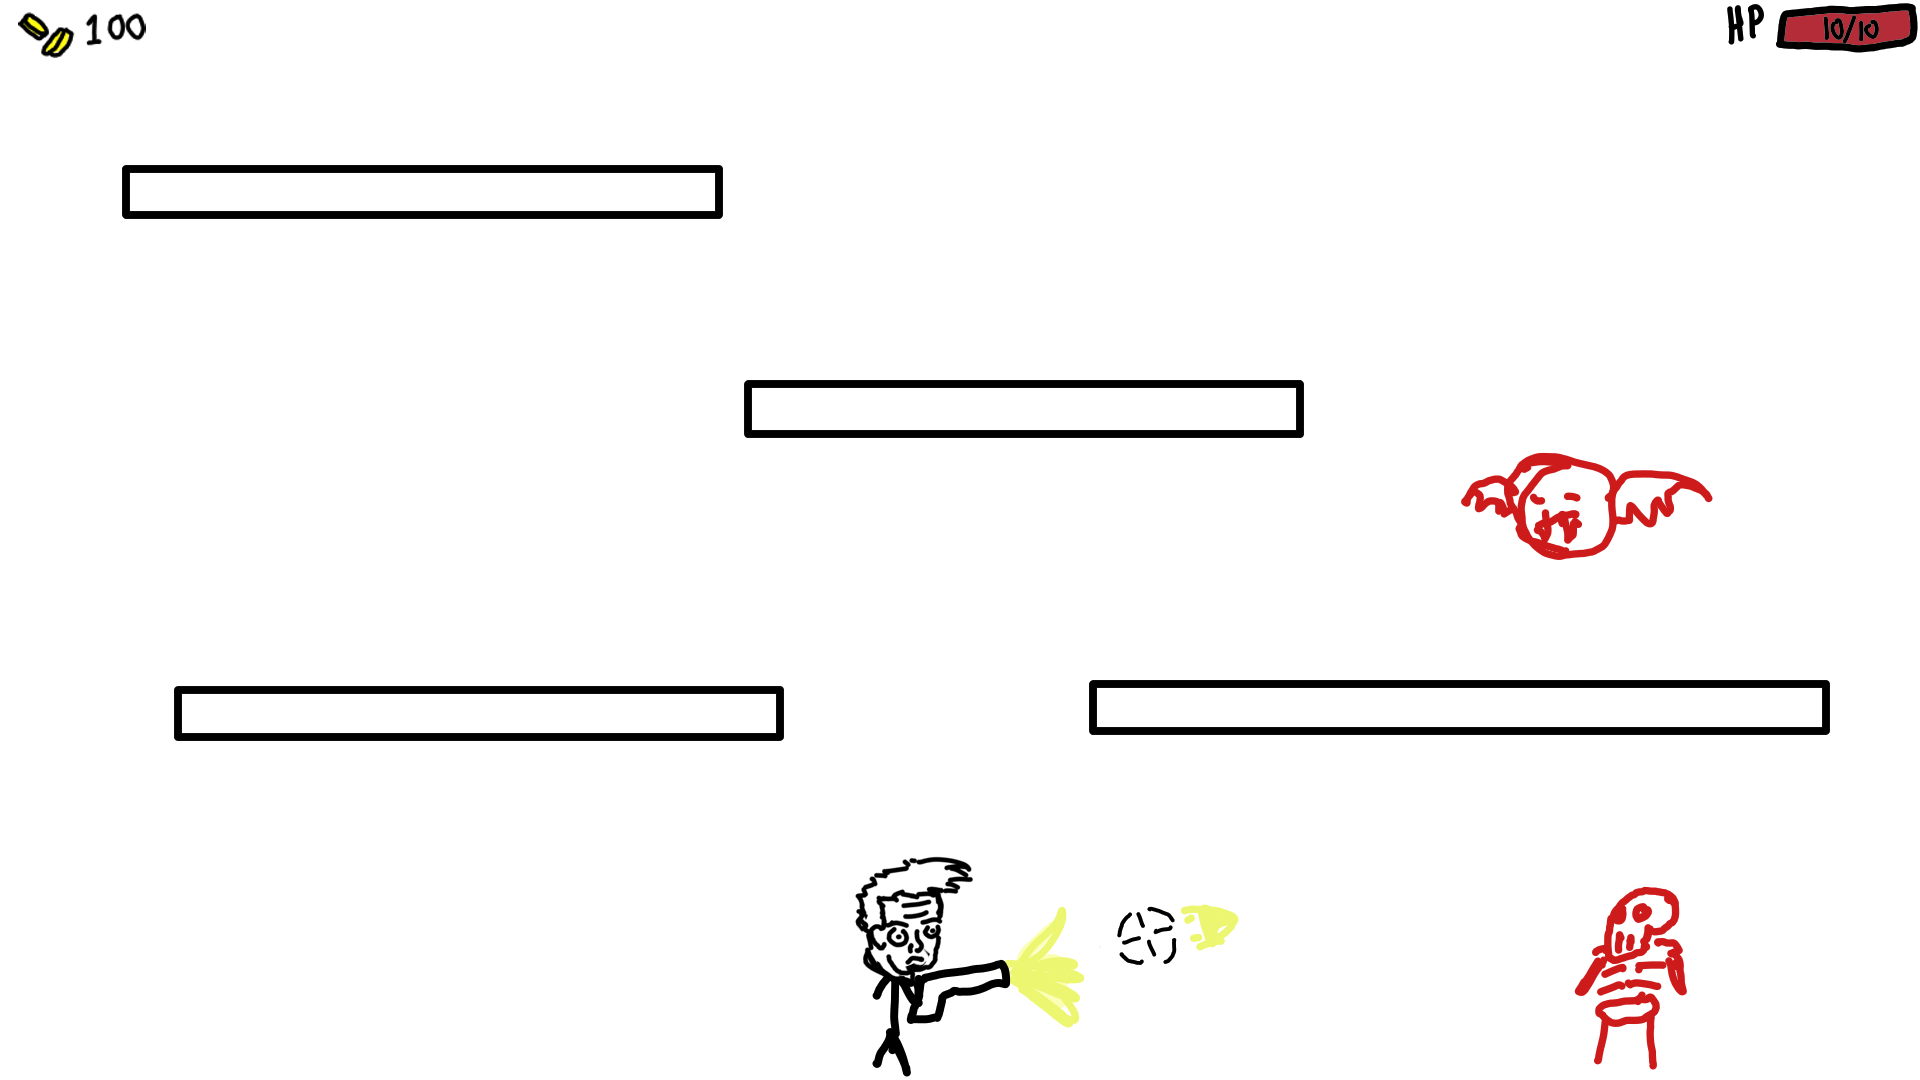
\includegraphics[width=15cm]{Graphic/main_concept.png}
             \caption{\label{fig:1} Ett exempel på en nivå, mitt i spelet.}
         \end{center}
\end{figure}

I figur \ref{fig:2} kan vi se ett enkelt exempel på en nivå efter alla fiender blivit besegrade. Det har skapats 3 uppgraderingar som kan köpas av spelaren. Därtill har dörren till nästa nivå skapats på höger sida.
\begin{figure}[H]
         \begin{center}
             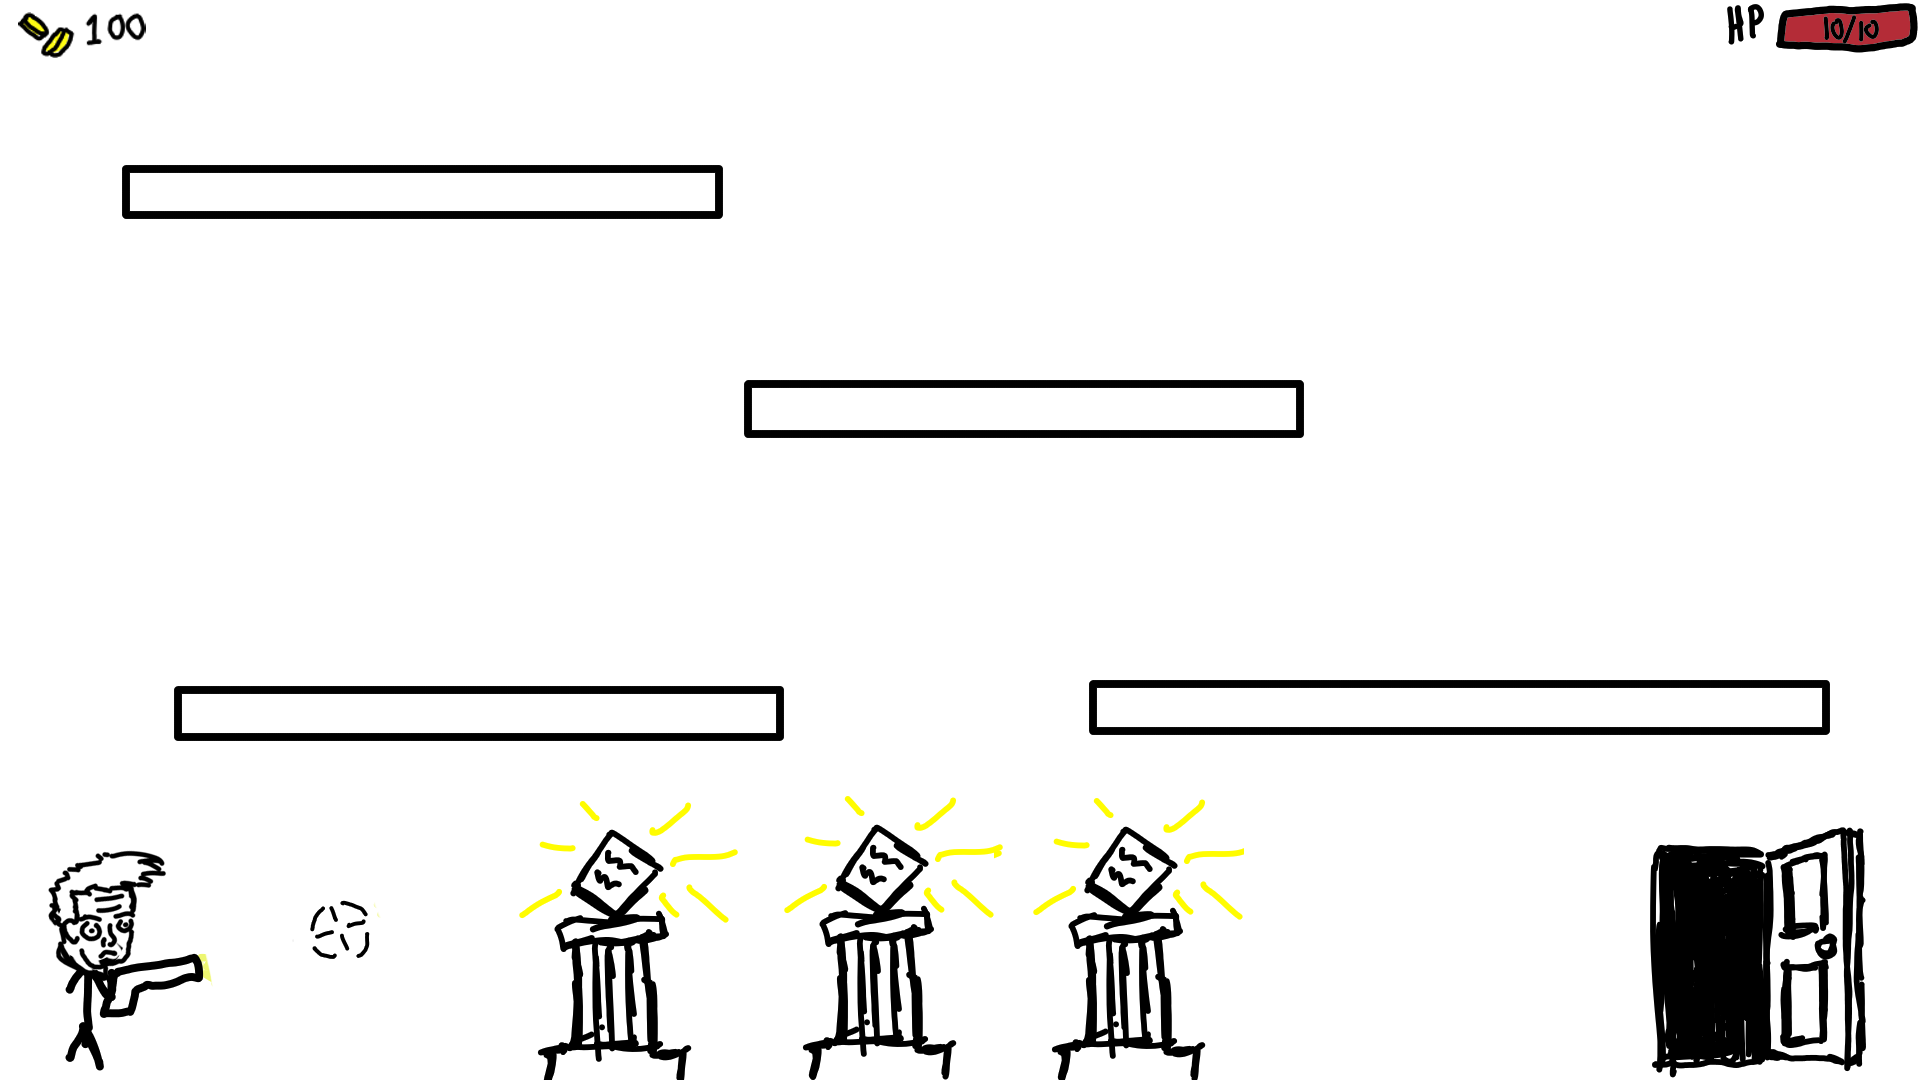
\includegraphics[width=15cm]{Graphic/win_concept.png}
             \caption{\label{fig:2} Ett exempel på en nivå, när alla fiender är besegrade.}
         \end{center}
\end{figure}

I figur \ref{fig:3} kan vi se ett enkelt exempel på en nivå när spelarens hälsa når 0. Vi kan se att hälsomätaren i höger hörn blivit tom då det röda skelettet (en fiende) nuddat spelarkaraktären. Vid förlust så stoppar spelet och ny grafik med orden 'GAME OVER' har lagts på skärmen. Spelaren uppmanas även till att starta om med 'E' tangenten.
\begin{figure}[H]
         \begin{center}
             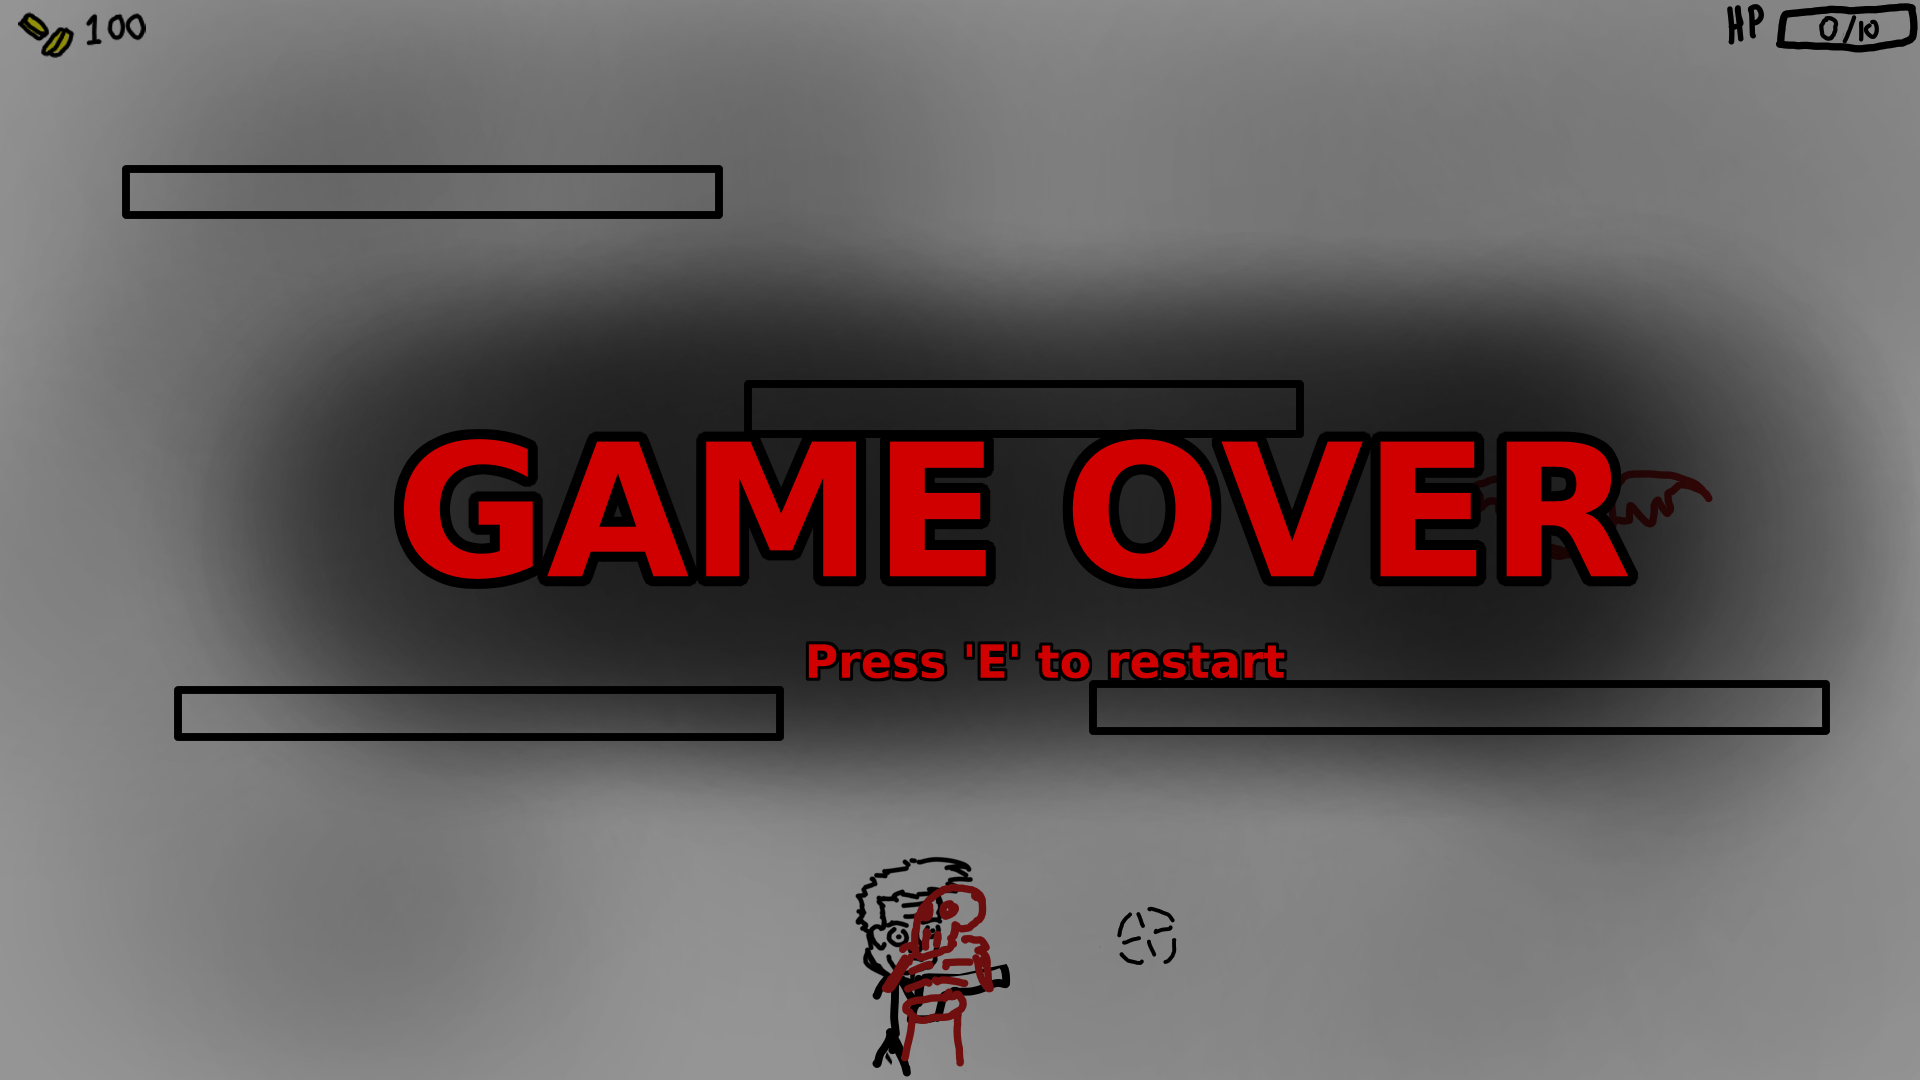
\includegraphics[width=15cm]{Graphic/lose_concept.png}
             \caption{\label{fig:3} Ett exempel på en nivå, när spelarens hälsa når 0.}
         \end{center}
\end{figure}

\section{Kravformulering}

\subsection{Ska-Krav}

\begin{enumerate}
\item Spelet ska innehålla en spelarkaraktär, en fiendetyp och projektiler.
\item Spelaren ska kunna flytta spelarkaraktären samt sikta och avfyra dess vapen enligt Tabell \ref{tab:1}.
\item Spelets fiender ska röra sig mot spelarkaraktären. När de kolliderar med spelarkaraktären ska denna ta skada.
\item Fiender ska ta skada när de träffas av spelarkaraktärens projektiler.
\item Spelarkaraktär och fiender ska ha hälsa som minskar när de tar skada. Når hälsan 0 ska karaktären raderas från spelplanen.
\item Når spelarens hälsa 0 ska spelet ta slut.
\item Att besegra fiender ska resultera i poäng som visas efter varje spelomgång.
\item Varje nivå ska skapa ett bestämt antal fiender som ökar utmed spelets gång.
\item När alla fiender på en nivå är besegrade ska spelaren kunna ta sig till nästa nivå. 
\item Spelets nivåer ska innehålla minst två olika spelplaner.
\item Spelaren ska se spelplanen ur ett tvådimensionellt sidoperspektiv.
\item Spelarkaraktären ska inte kunna röra sig utanför spelplanens gränser och kunna stå på plattformar.


\subsection{Bör-Krav}

\item Spelaren ska kunna samla pengar som fiender skapar när de dör.
\item Spelarkaraktärens egenskaper ska kunna förändras genom att få uppgraderingar. 
\item Spelaren ska kunna spendera pengar för att få uppgraderingar mellan nivåer.
\item Samlade pengar ska sparas mellan varje nivå och spenderade spengar ska subtraheras från totalen.
\end{enumerate}

\section{Kravuppfyllelse}
\begin{itemize}
\item Spelet ska simulera en värld som innehåller olika typer av objekt. Objekten ska ha olika beteenden och röra sig i världen och agera på olika sätt när de möter andra objekt.

Uppfylls av krav: 1, 2, 3
\item Det måste finnas minst tre olika typer av objekt och det ska finnas flera instanser av minst två av dessa. T.ex ett spelarobjekt och många instanser av två olika slags fiendeobjekt.

Uppfylls av krav: 1
\item Ett beteende som måste finnas med är att figurerna ska röra sig över skärmen. Rörelsen kan följa ett mönster och/eller vara slumpmässig. Minst ett objekt, utöver spelaren ska ha någon typ av rörelse.

Uppfylls av krav: 3
\item En figur ska styras av spelaren, antingen med tangentbordet eller med musen. Du kan även göra ett spel där man spelar två stycken genom att dela på tangentbordet (varje spelare använder olika tangenter). Då styr man var sin figur.

Uppfylls av krav: 2
\item Grafiken ska vara tvådimensionell.

Uppfylls av krav: 11
\item Världen (spelplanen) kan antas vara lika stor som fönstret (du kan göra en större spelplan med scrollning, men det blir lite krångligare).

Uppfylls av krav: 11
\item Det ska finnas kollisionshantering, det vill säga, det ska hända olika saker när objekten möter varandra, de ska påverka varandra på något sätt. 

Uppfylls av krav: 3, 4, 12
\item Det ska vara enkelt att lägga till eller ändra banor i spelet. Detta kan exempelvis lösas genom att läsa in banor från en fil (lite som i Sokoban-labben i TDP002), eller genom att ha funktioner i programkoden som bygger upp en datastruktur som definierar en bana.

Uppfylls av krav: 10
\item Spelet måste upplevas som ett sammanhängande spel som går att spela!

Då alla ska-krav är uppfyllda bör programmet upplevas som ett spel då det har en början, ett slut, mål och spelmekaniker. 
\end{itemize}

\end{document}
